\documentclass[../AnalysisNoteJBuxton.tex]{subfiles}
\begin{document}

\subsubsection{\texorpdfstring{$\bar{\Lambda}$K$^{0}_{S}$}{TEXT} Residuals}
\label{Residuals_ALamK0}

\begin{figure}[h]
  \centering
  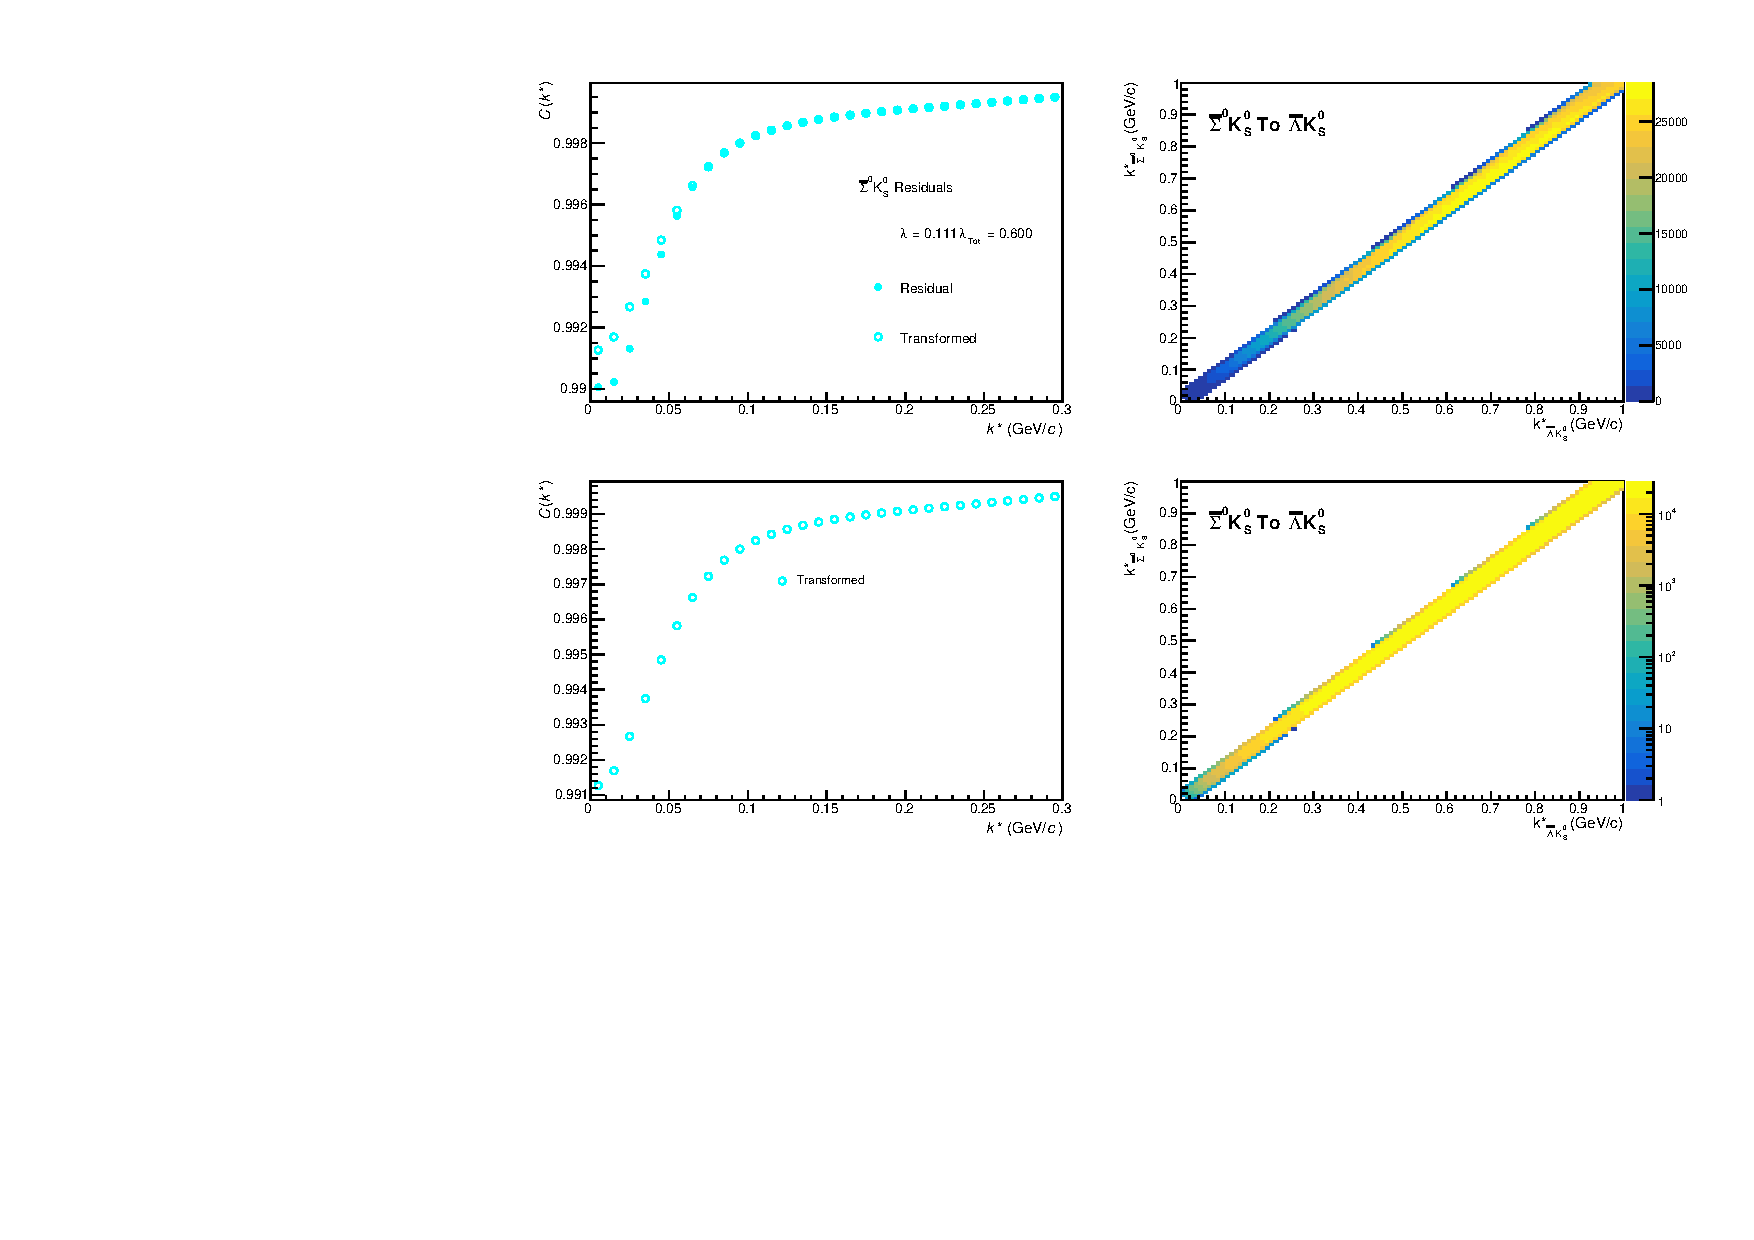
\includegraphics[width=\textwidth]{9_AdditionalFigures/Figures/Residuals/ALamK0/Residuals_ALamK0_0010_ASig0K0_MomResCrctn_NonFlatBgdCrctn_SingleLamParam_10Res_PrimMaxDecay4fm_UsingXiDataAndCoulombOnly.pdf}
  \caption[Residuals: $\bar{\Sigma}^{0}$K$^{0}_{S}$ to $\bar{\Lambda}$K$^{0}_{S}$ (0-10\% Centrality)]{Residuals: $\bar{\Sigma}^{0}$K$^{0}_{S}$ to $\bar{\Lambda}$K$^{0}_{S}$ (0-10\% Centrality)}
  \label{fig:Res_ALamK0_0010_ASig0K0}
\end{figure}


\begin{figure}[h]
  \centering
  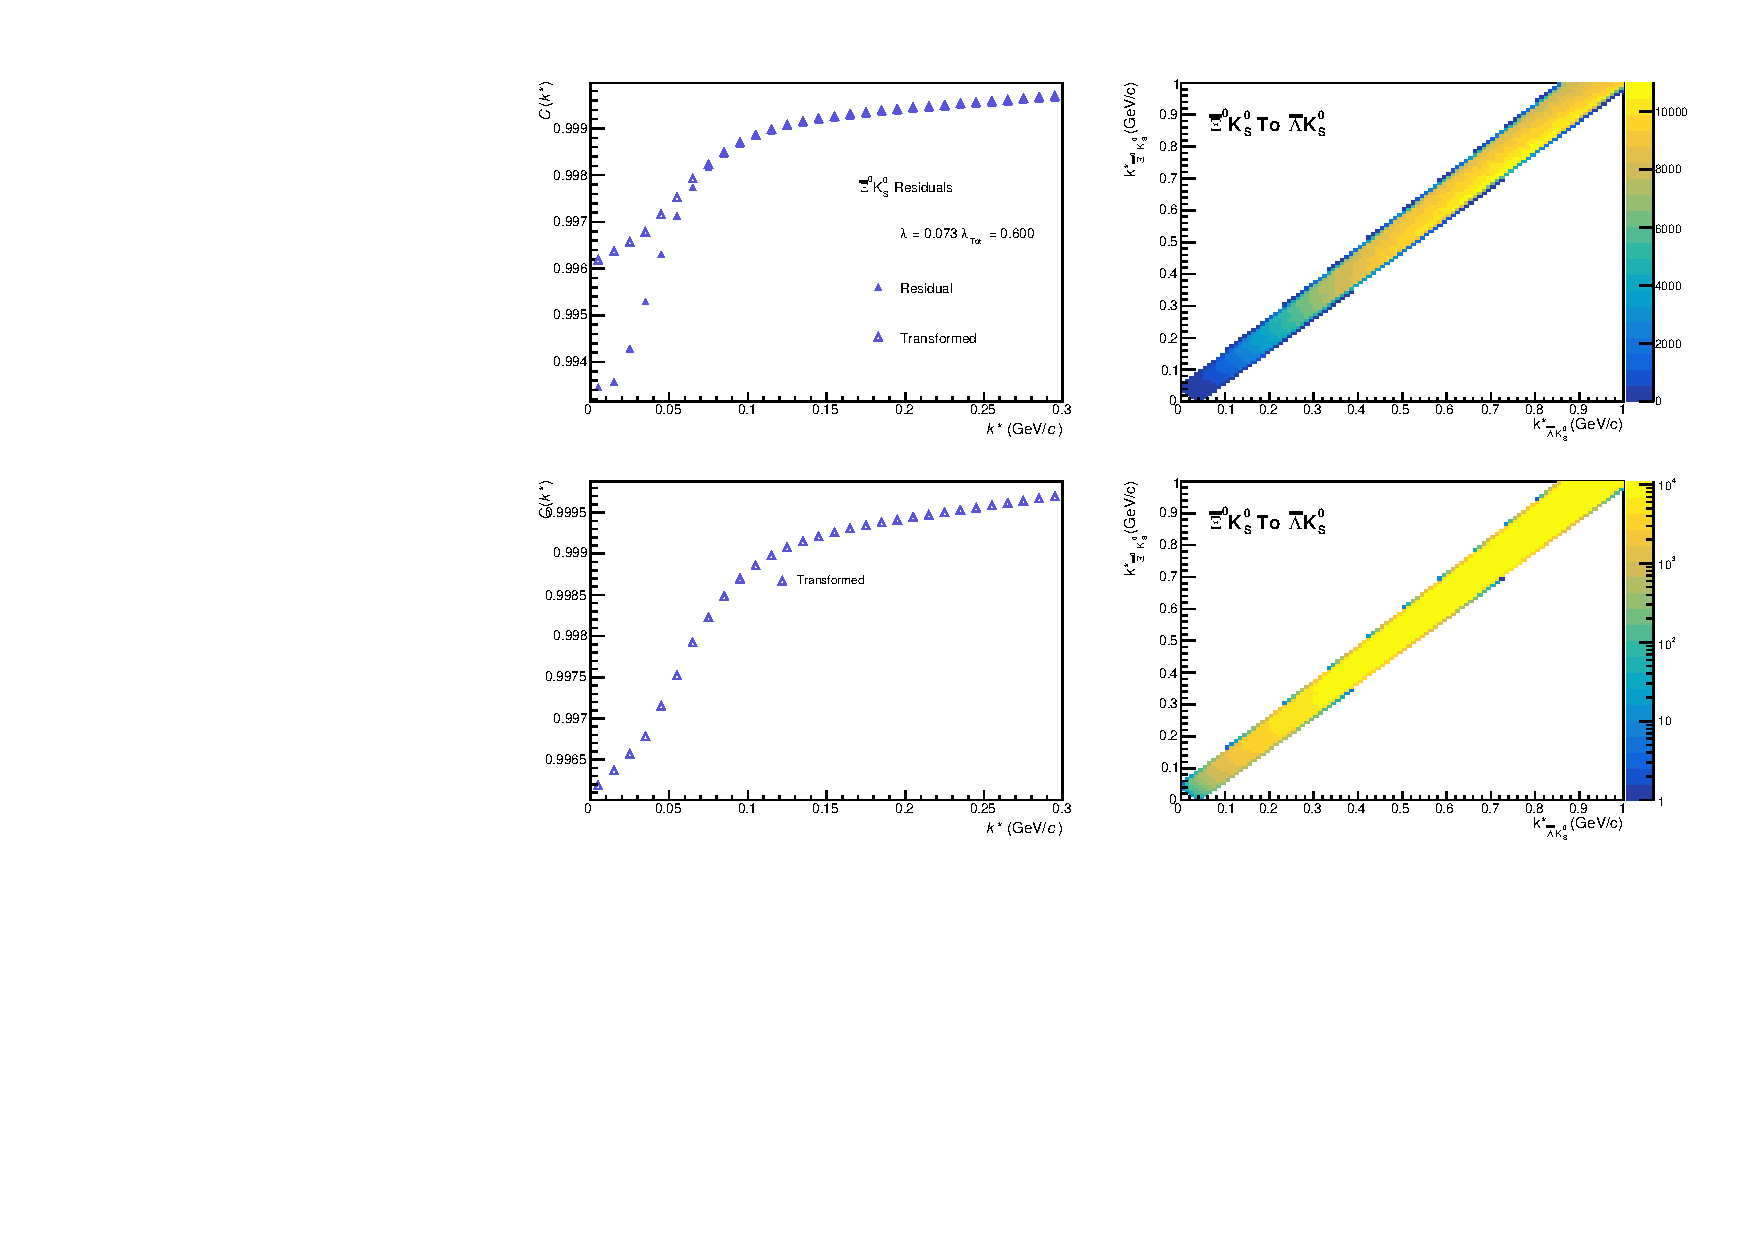
\includegraphics[width=\textwidth]{9_AdditionalFigures/Figures/Residuals/ALamK0/Residuals_ALamK0_0010_AXi0K0_MomResCrctn_NonFlatBgdCrctn_SingleLamParam_10Res_PrimMaxDecay4fm_UsingXiDataAndCoulombOnly.pdf}
  \caption[Residuals: $\bar{\Xi}^{0}$K$^{0}_{S}$ to $\bar{\Lambda}$K$^{0}_{S}$ (0-10\% Centrality)]{Residuals: $\bar{\Xi}^{0}$K$^{0}_{S}$ to $\bar{\Lambda}$K$^{0}_{S}$ (0-10\% Centrality)}
  \label{fig:Res_ALamK0_0010_AXi0K0}
\end{figure}


\begin{figure}[h]
  \centering
  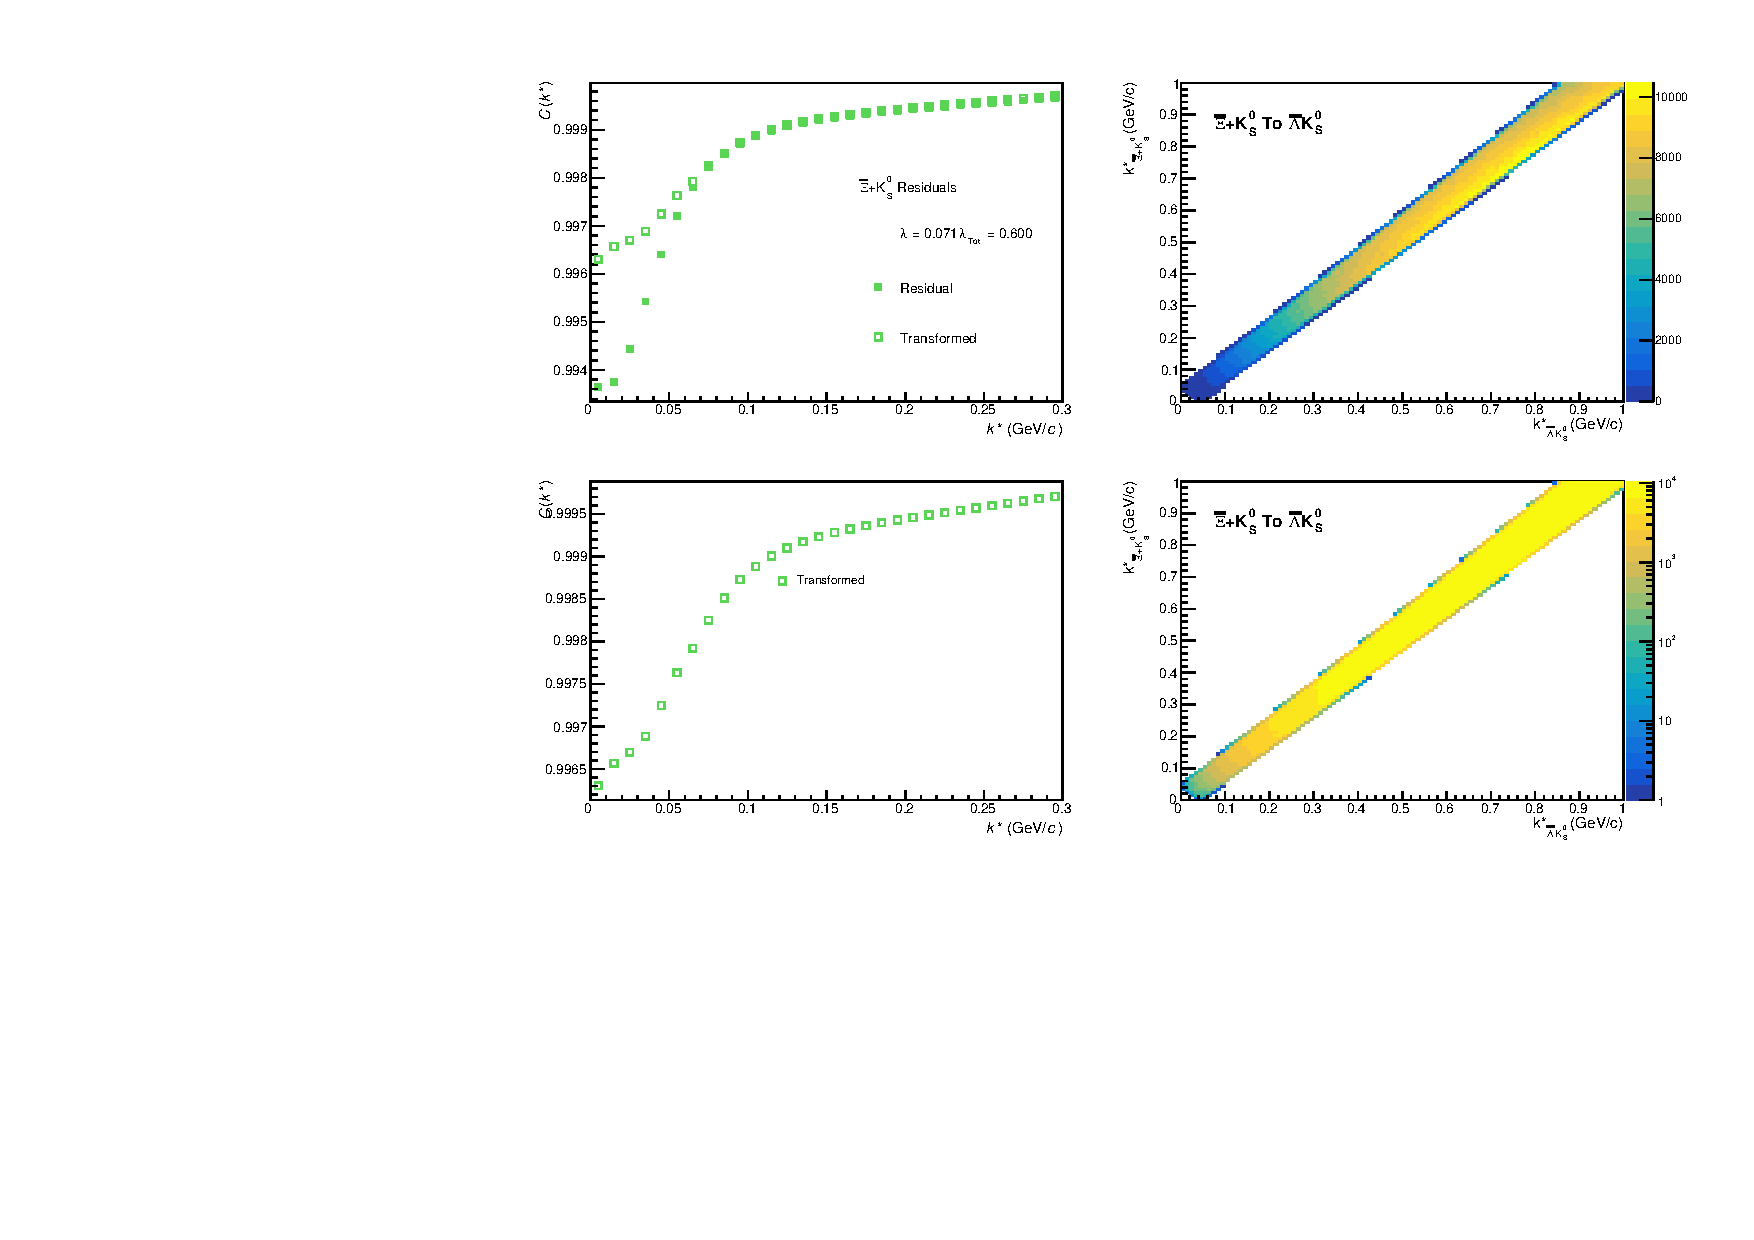
\includegraphics[width=\textwidth]{9_AdditionalFigures/Figures/Residuals/ALamK0/Residuals_ALamK0_0010_AXiK0_MomResCrctn_NonFlatBgdCrctn_SingleLamParam_10Res_PrimMaxDecay4fm_UsingXiDataAndCoulombOnly.pdf}
  \caption[Residuals: $\bar{\Xi}^{+}$K$^{0}_{S}$ to $\bar{\Lambda}$K$^{0}_{S}$ (0-10\% Centrality)]{Residuals: $\bar{\Xi}^{+}$K$^{0}_{S}$ to $\bar{\Lambda}$K$^{0}_{S}$ (0-10\% Centrality)}
  \label{fig:Res_ALamK0_0010_AXiCK0}
\end{figure}


\begin{figure}[h]
  \centering
  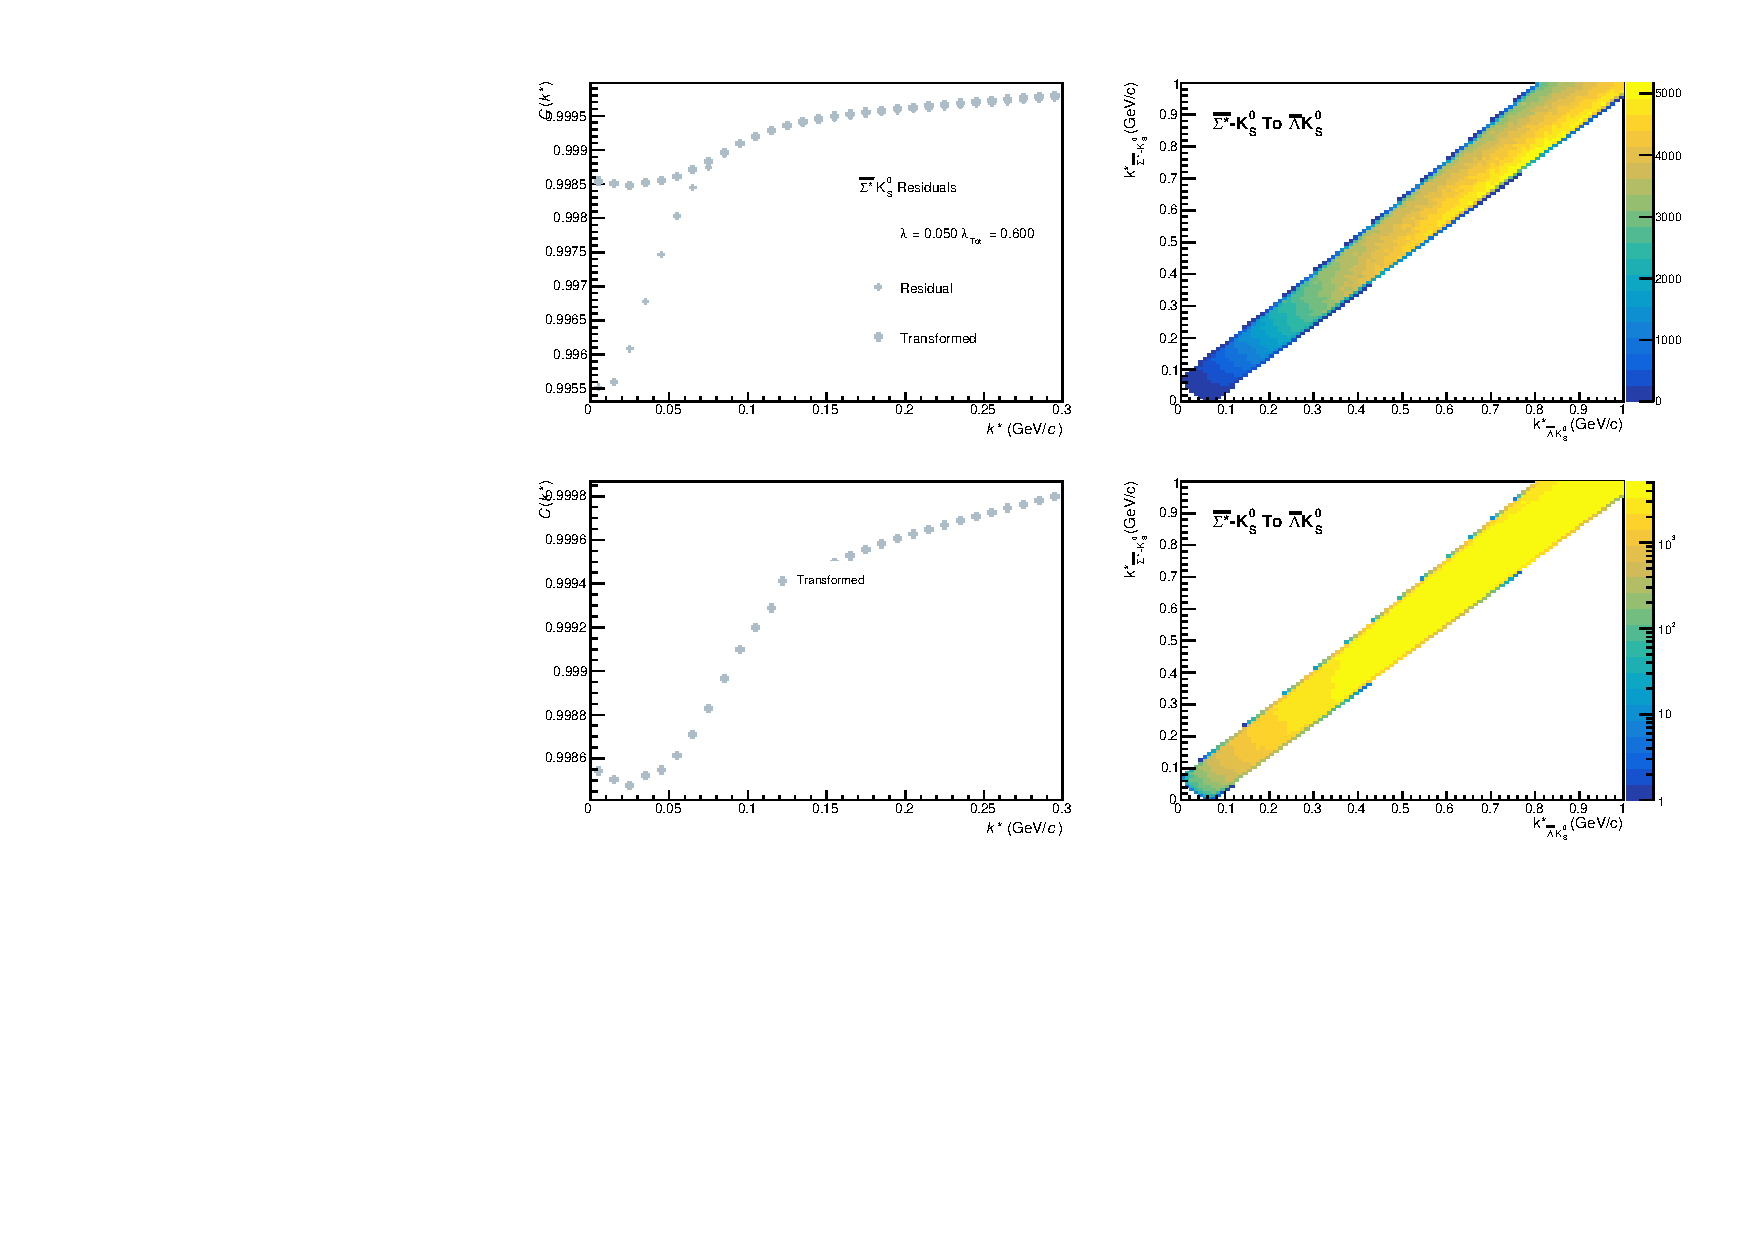
\includegraphics[width=\textwidth]{9_AdditionalFigures/Figures/Residuals/ALamK0/Residuals_ALamK0_0010_ASigStMK0_MomResCrctn_NonFlatBgdCrctn_SingleLamParam_10Res_PrimMaxDecay4fm_UsingXiDataAndCoulombOnly.pdf}
  \caption[Residuals: $\bar{\Sigma}^{*-}$K$^{0}_{S}$ to $\bar{\Lambda}$K$^{0}_{S}$ (0-10\% Centrality)]{Residuals: $\bar{\Sigma}^{*-}$K$^{0}_{S}$ to $\bar{\Lambda}$K$^{0}_{S}$ (0-10\% Centrality)}
  \label{fig:Res_ALamK0_0010_ASigStMK0}
\end{figure}

\begin{figure}[h]
  \centering
  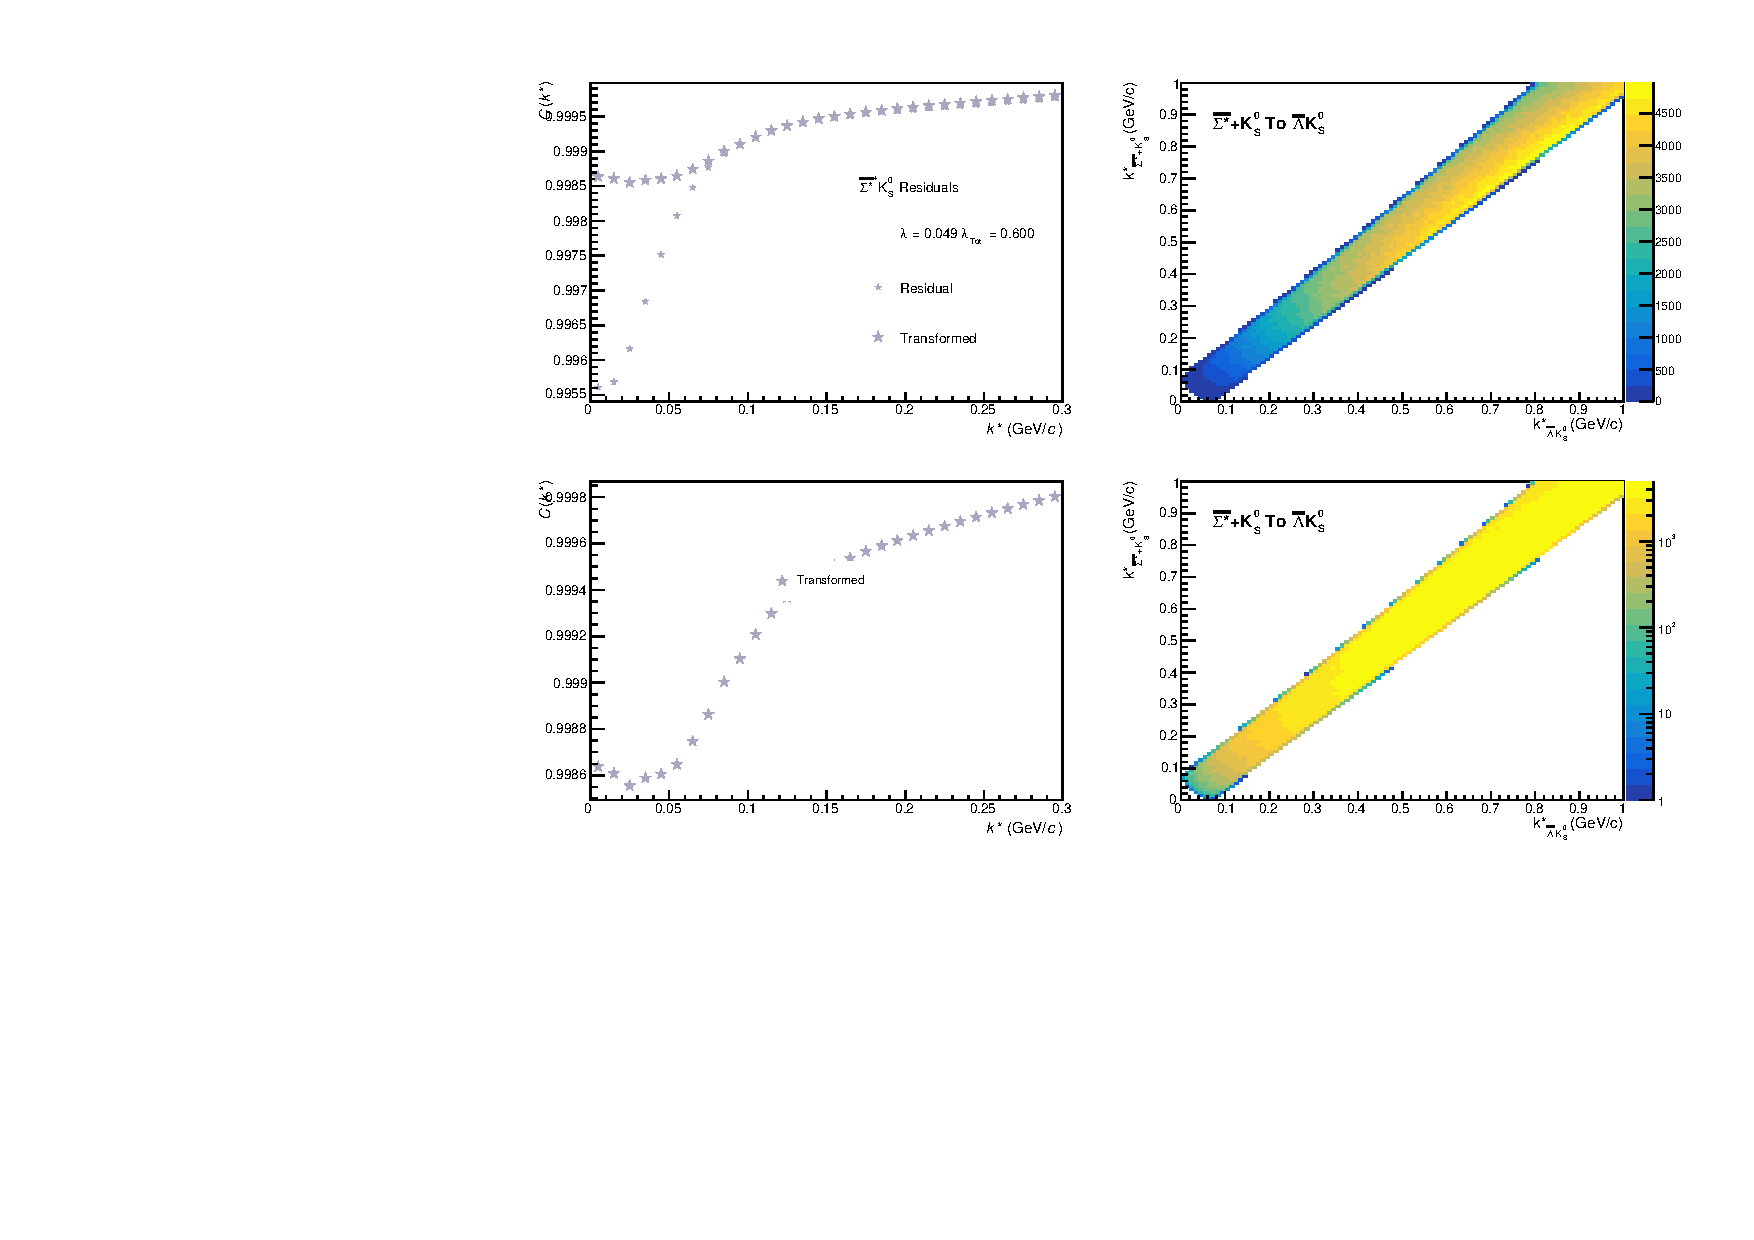
\includegraphics[width=\textwidth]{9_AdditionalFigures/Figures/Residuals/ALamK0/Residuals_ALamK0_0010_ASigStPK0_MomResCrctn_NonFlatBgdCrctn_SingleLamParam_10Res_PrimMaxDecay4fm_UsingXiDataAndCoulombOnly.pdf}
  \caption[Residuals: $\bar{\Sigma}^{*+}$K$^{0}_{S}$ to $\bar{\Lambda}$K$^{0}_{S}$ (0-10\% Centrality)]{Residuals: $\bar{\Sigma}^{*+}$K$^{0}_{S}$ to $\bar{\Lambda}$K$^{0}_{S}$ (0-10\% Centrality)}
  \label{fig:Res_ALamK0_0010_ASigStPK0}
\end{figure}

\begin{figure}[h]
  \centering
  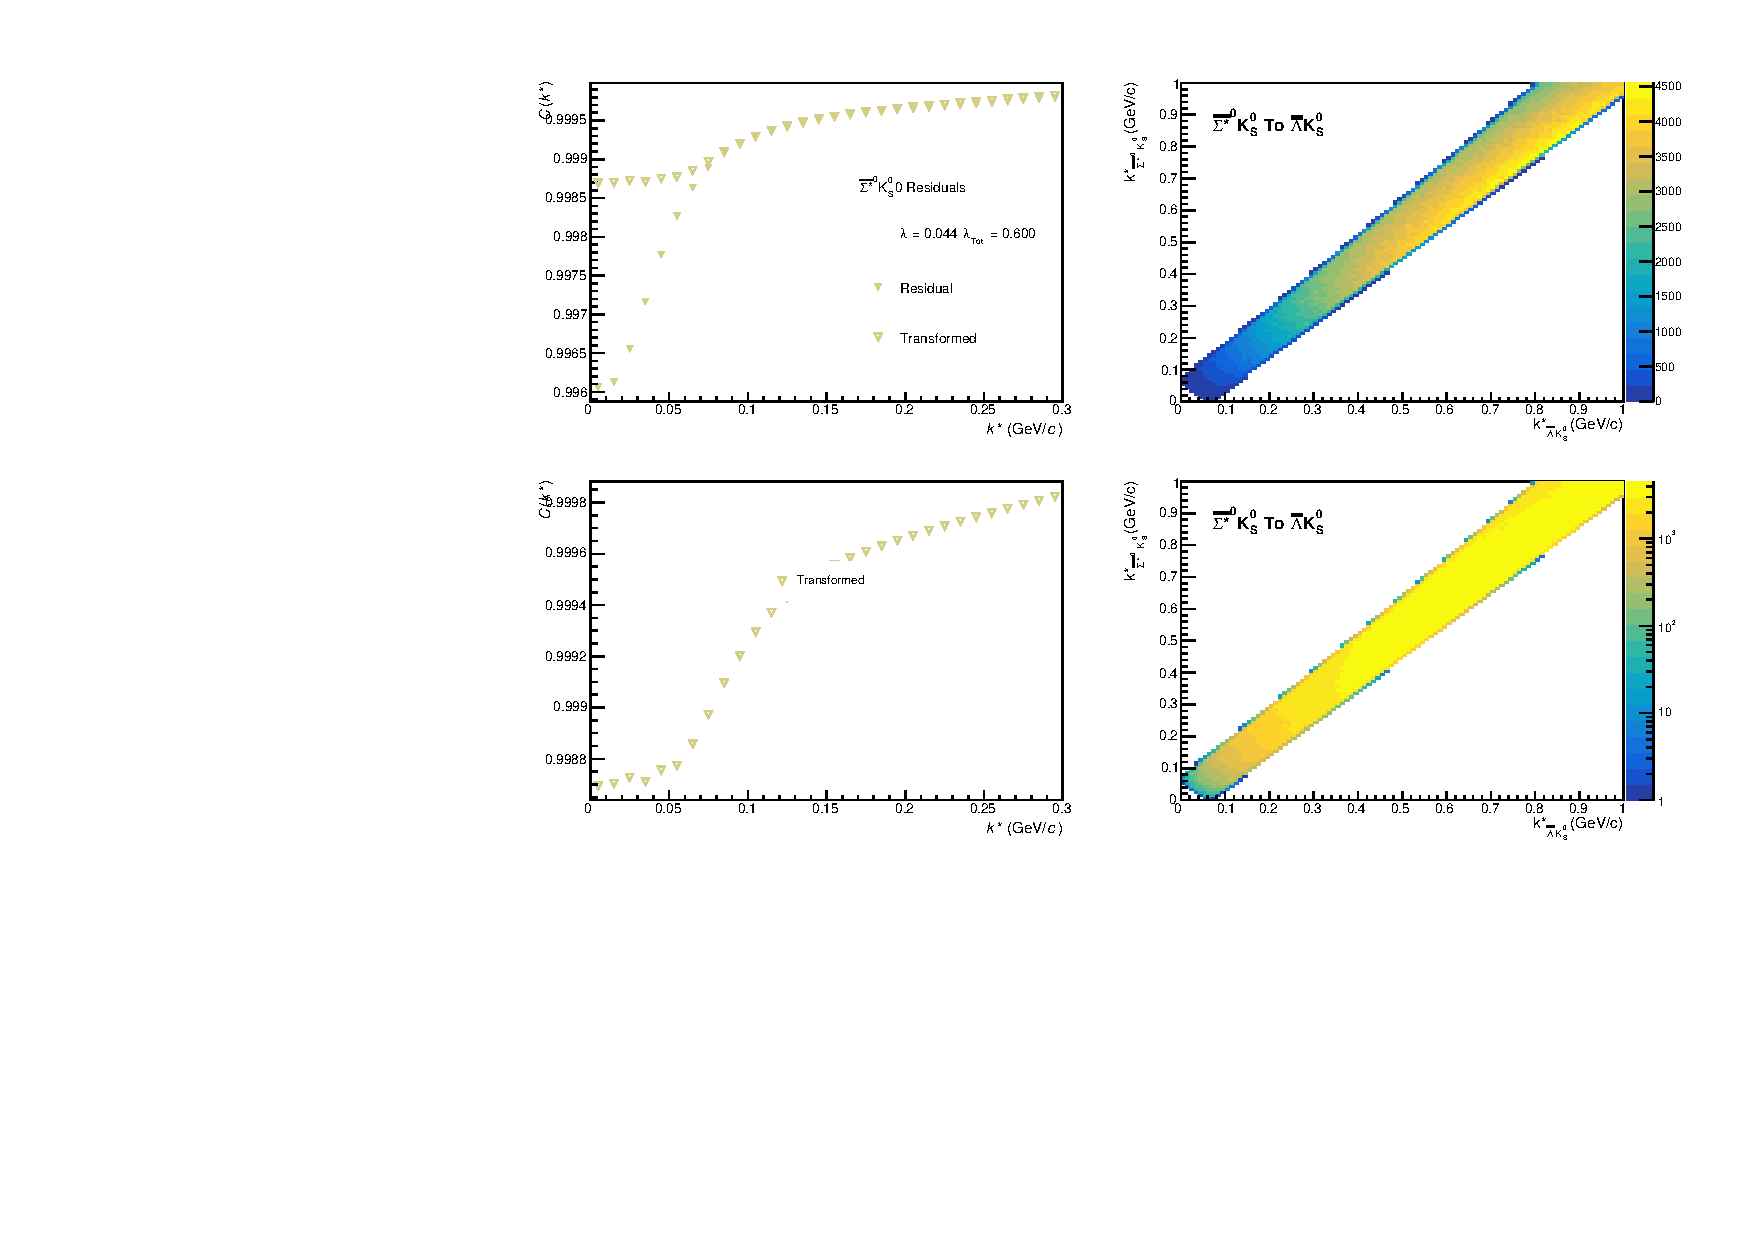
\includegraphics[width=\textwidth]{9_AdditionalFigures/Figures/Residuals/ALamK0/Residuals_ALamK0_0010_ASigSt0K0_MomResCrctn_NonFlatBgdCrctn_SingleLamParam_10Res_PrimMaxDecay4fm_UsingXiDataAndCoulombOnly.pdf}
  \caption[Residuals: $\bar{\Sigma}^{*0}$K$^{0}_{S}$ to $\bar{\Lambda}$K$^{0}_{S}$ (0-10\% Centrality)]{Residuals: $\bar{\Sigma}^{*0}$K$^{0}_{S}$ to $\bar{\Lambda}$K$^{0}_{S}$ (0-10\% Centrality)}
  \label{fig:Res_ALamK0_0010_ASigSt0K0}
\end{figure}


\begin{figure}[h]
  \centering
  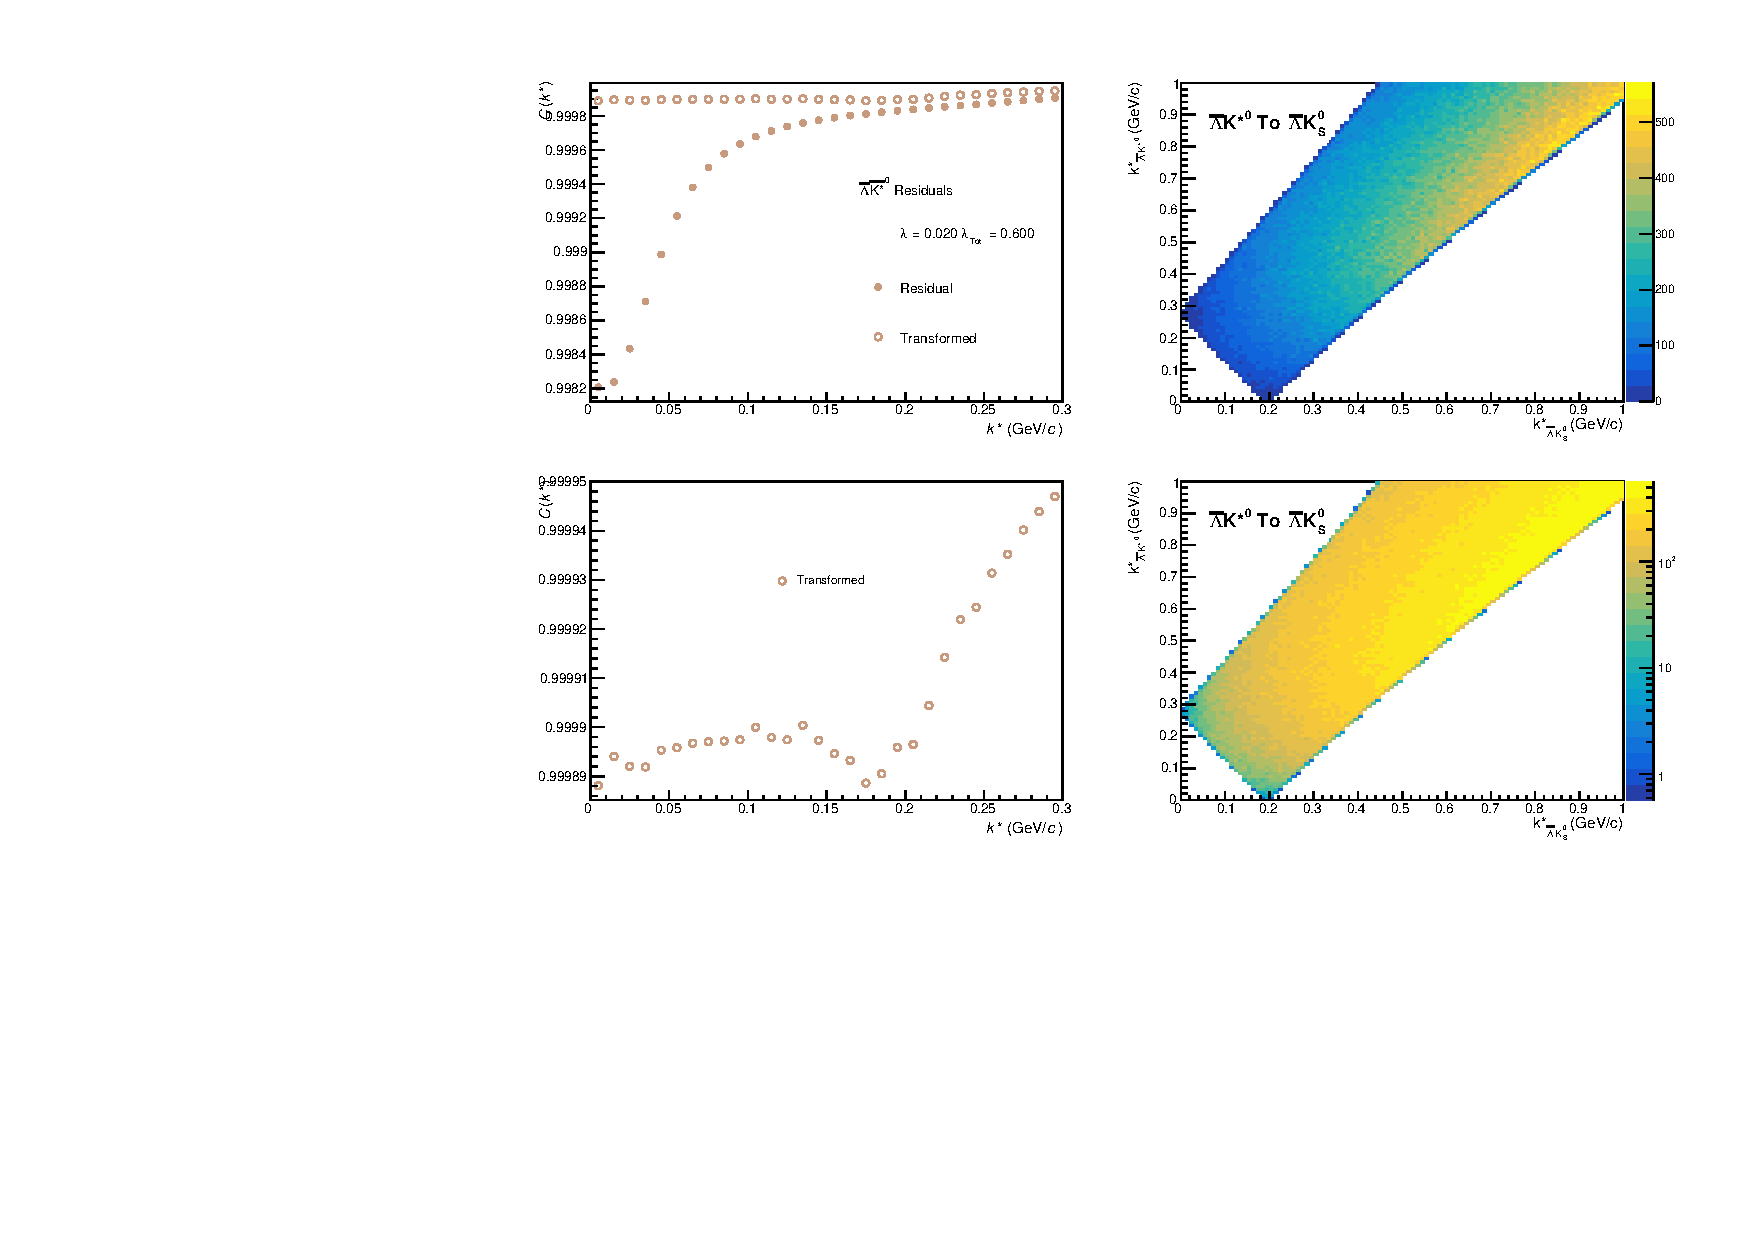
\includegraphics[width=\textwidth]{9_AdditionalFigures/Figures/Residuals/ALamK0/Residuals_ALamK0_0010_ALamKSt0ToALamK0_MomResCrctn_NonFlatBgdCrctn_SingleLamParam_10Res_PrimMaxDecay4fm_UsingXiDataAndCoulombOnly.pdf}
  \caption[Residuals: $\bar{\Lambda}$K$^{*0}$ to $\bar{\Lambda}$K$^{0}_{S}$ (0-10\% Centrality)]{Residuals: $\bar{\Lambda}$K$^{*0}$ to $\bar{\Lambda}$K$^{0}_{S}$ (0-10\% Centrality)}
  \label{fig:Res_ALamK0_0010_ALamKSt0}
\end{figure}


\begin{figure}[h]
  \centering
  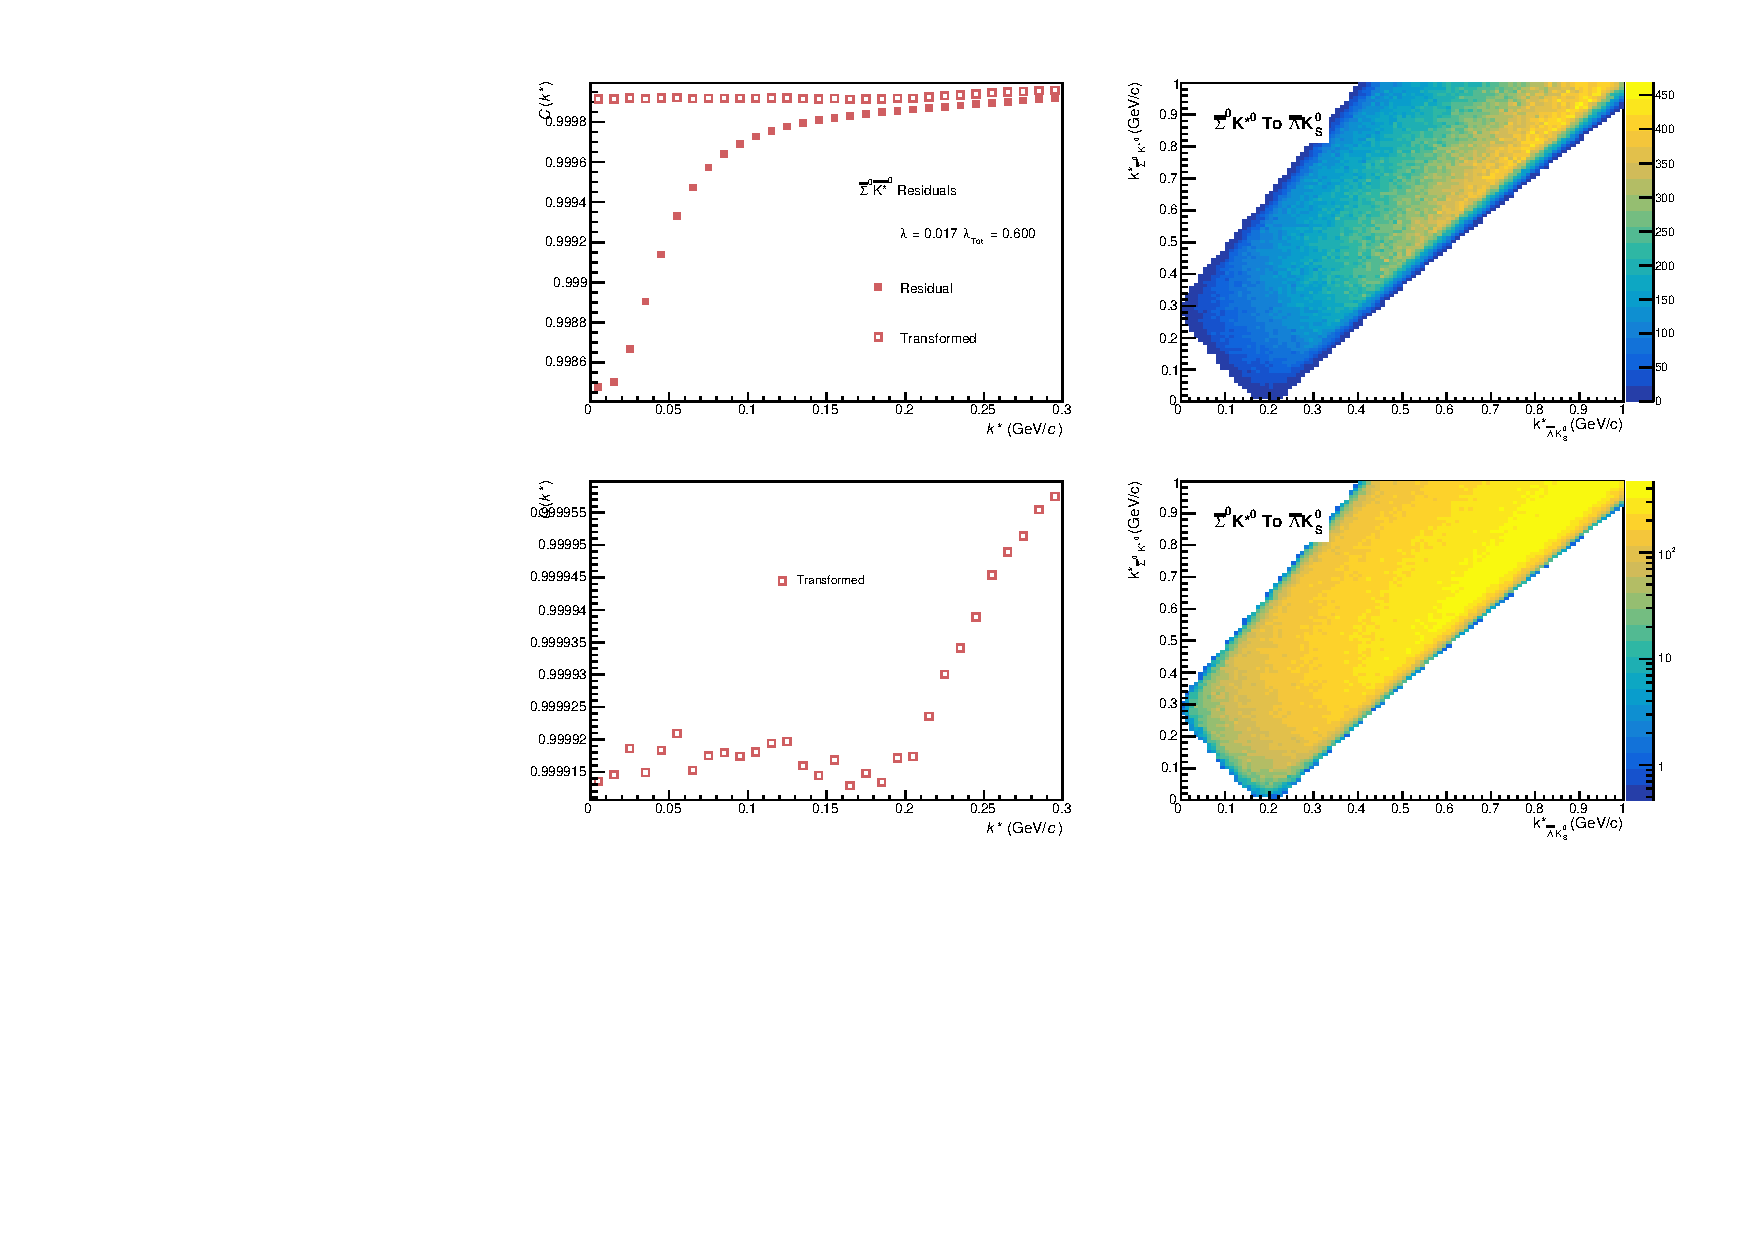
\includegraphics[width=\textwidth]{9_AdditionalFigures/Figures/Residuals/ALamK0/Residuals_ALamK0_0010_ASigma0KSt0ToALamK0_MomResCrctn_NonFlatBgdCrctn_SingleLamParam_10Res_PrimMaxDecay4fm_UsingXiDataAndCoulombOnly.pdf}
  \caption[Residuals: $\bar{\Sigma}^{0}$K$^{*0}$ to $\bar{\Lambda}$K$^{0}_{S}$ (0-10\% Centrality)]{Residuals: $\bar{\Sigma}^{0}$K$^{*0}$ to $\bar{\Lambda}$K$^{0}_{S}$ (0-10\% Centrality)}
  \label{fig:Res_ALamK0_0010_ASig0KSt0}
\end{figure}


\begin{figure}[h]
  \centering
  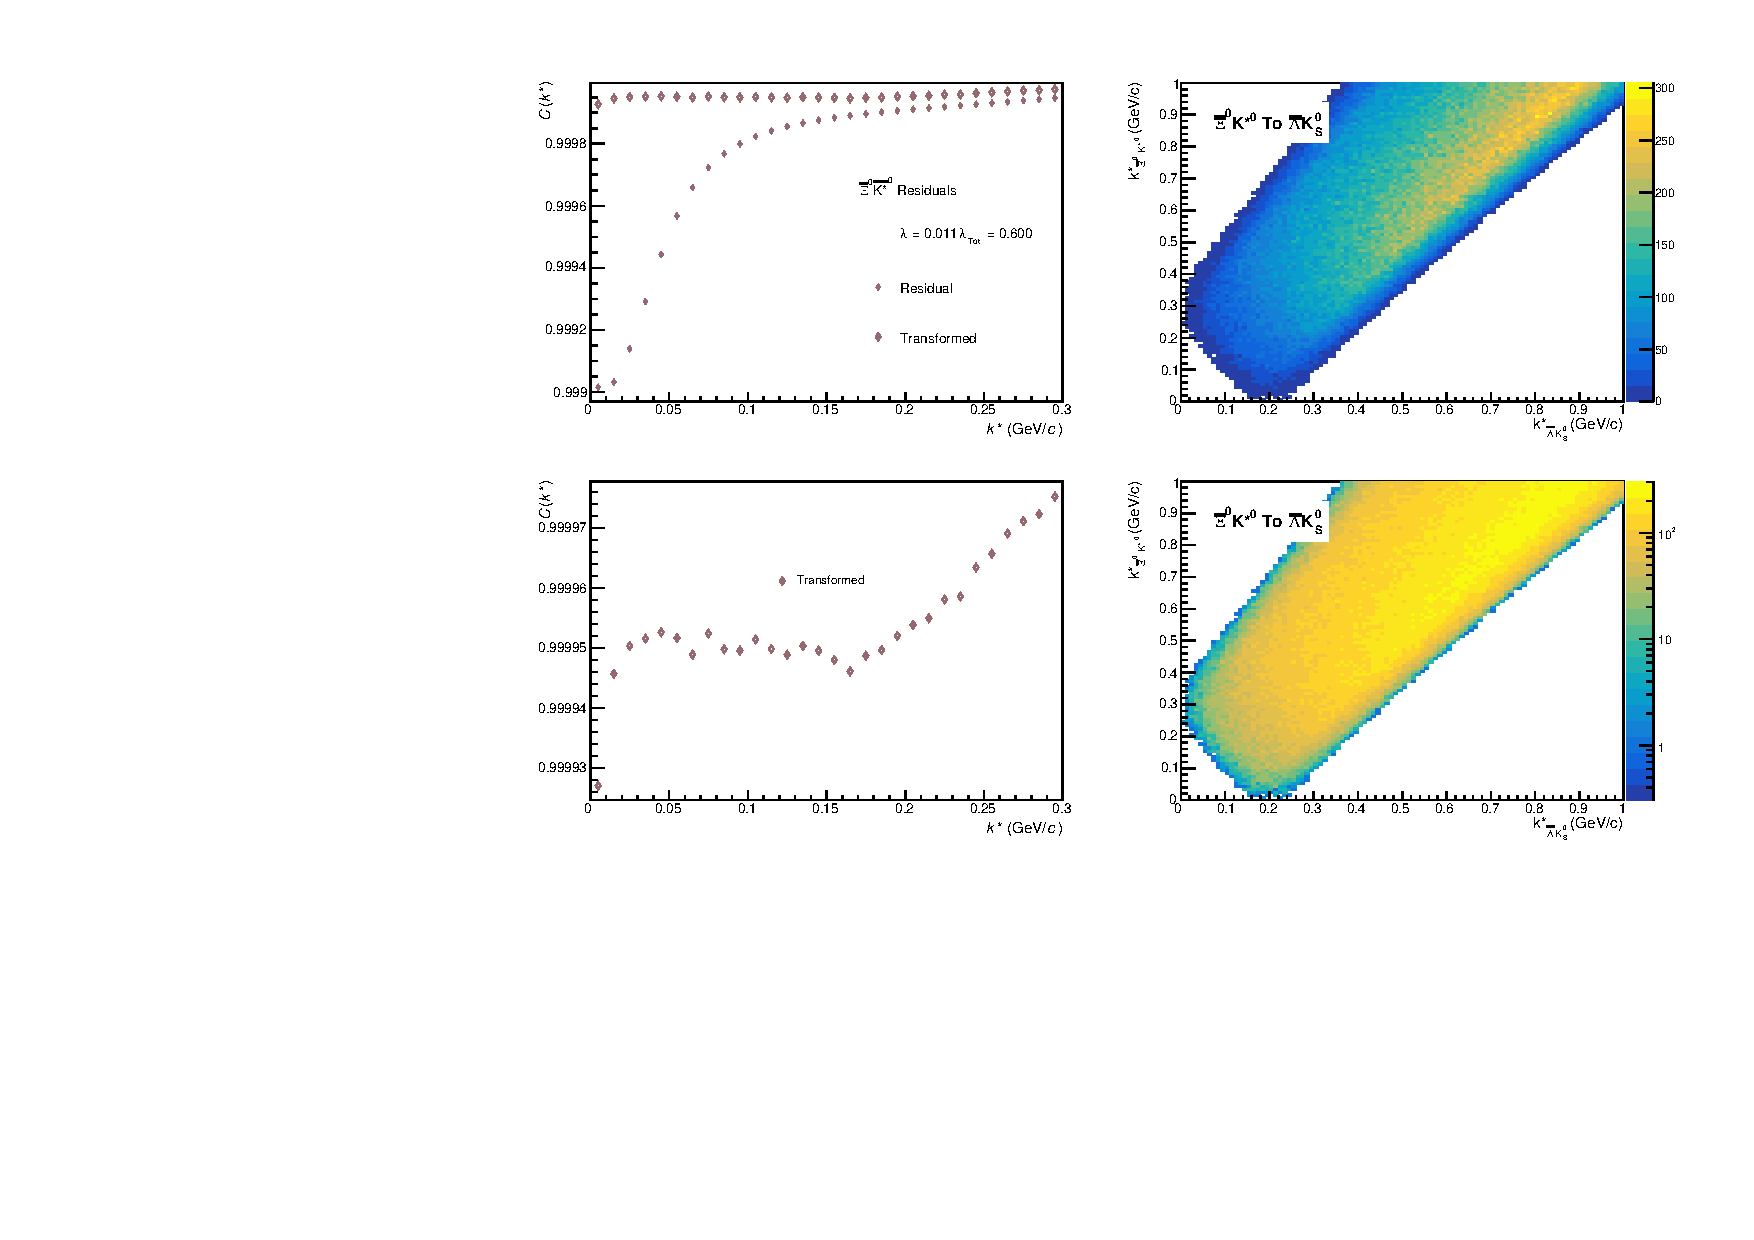
\includegraphics[width=\textwidth]{9_AdditionalFigures/Figures/Residuals/ALamK0/Residuals_ALamK0_0010_AXi0KSt0ToALamK0_MomResCrctn_NonFlatBgdCrctn_SingleLamParam_10Res_PrimMaxDecay4fm_UsingXiDataAndCoulombOnly.pdf}
  \caption[Residuals: $\bar{\Xi}^{0}$K$^{*0}$ to $\bar{\Lambda}$K$^{0}_{S}$ (0-10\% Centrality)]{Residuals: $\bar{\Xi}^{0}$K$^{*0}$ to $\bar{\Lambda}$K$^{0}_{S}$ (0-10\% Centrality)}
  \label{fig:Res_ALamK0_0010_AXi0KSt0}
\end{figure}

\begin{figure}[h]
  \centering
  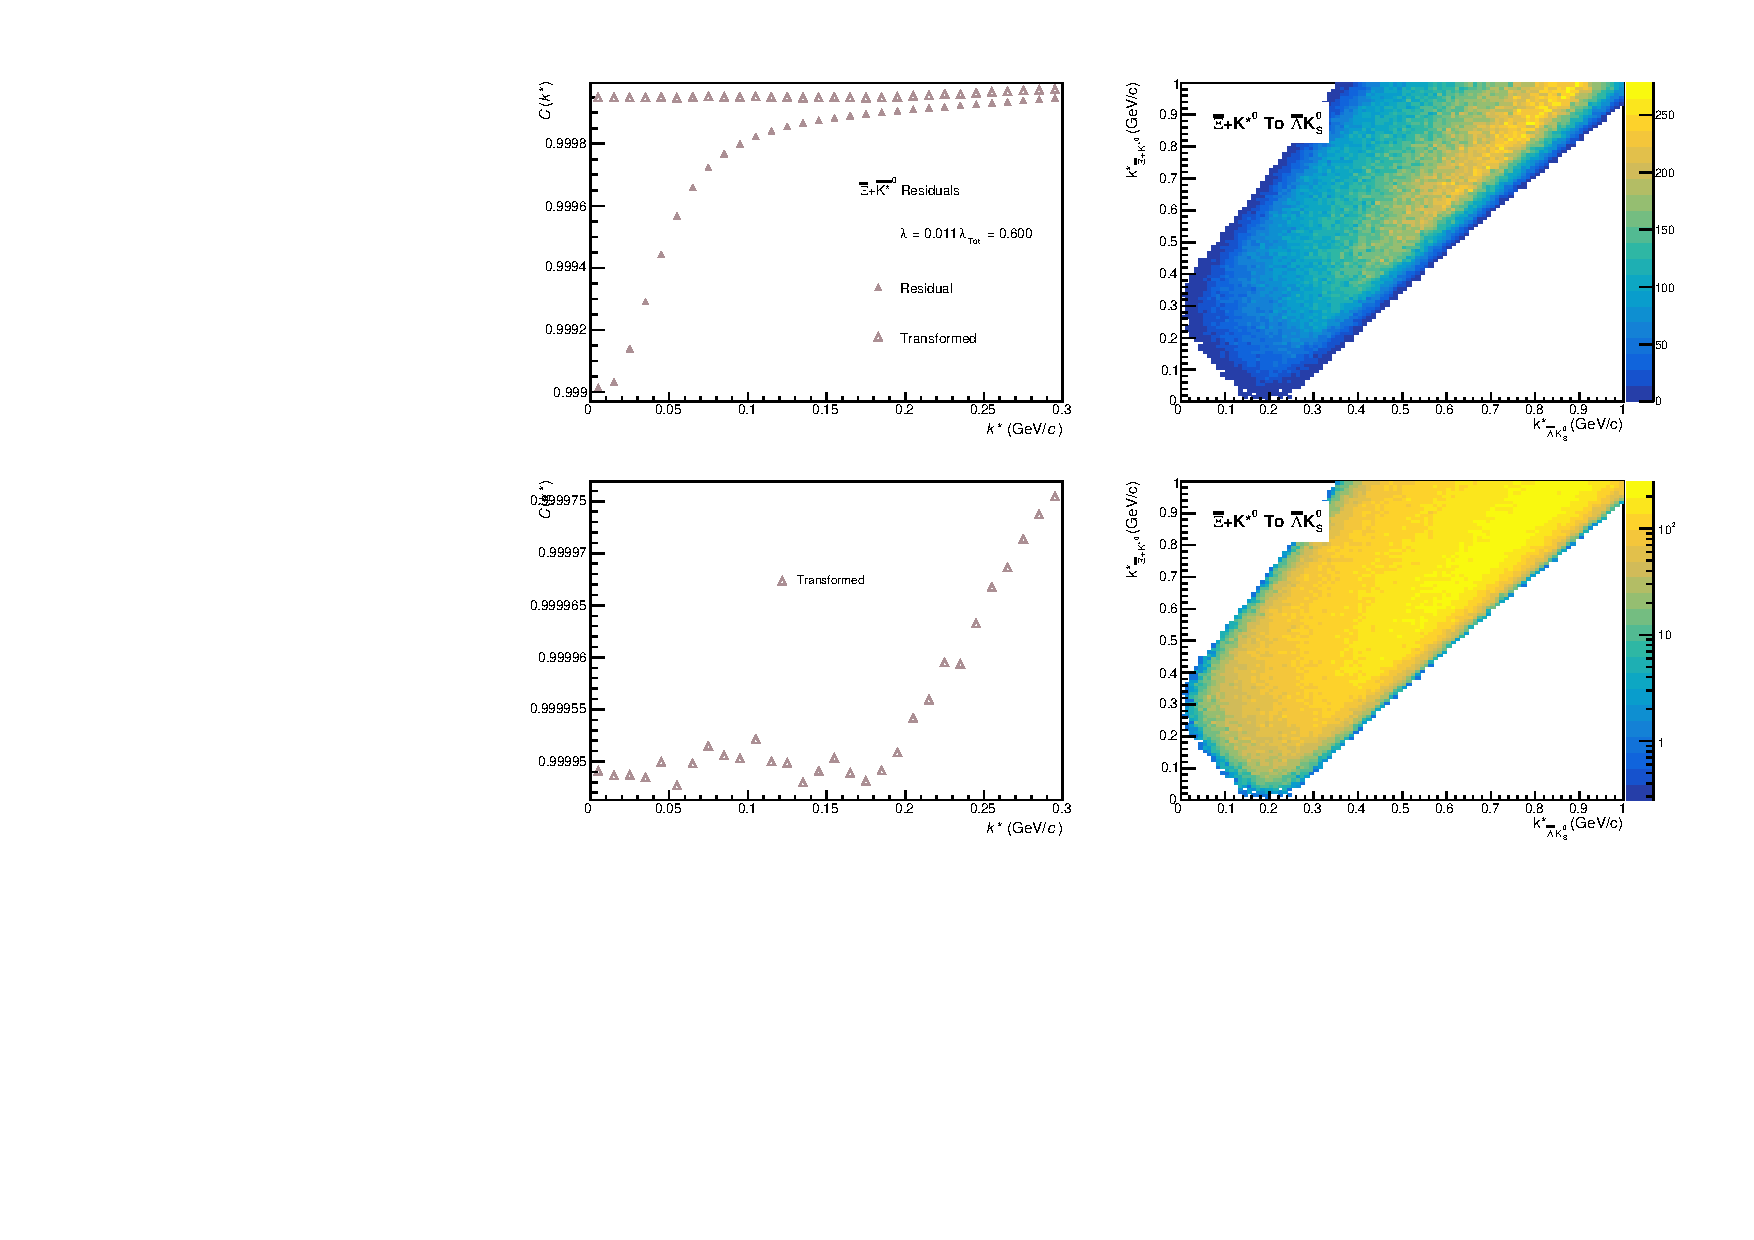
\includegraphics[width=\textwidth]{9_AdditionalFigures/Figures/Residuals/ALamK0/Residuals_ALamK0_0010_AXiKSt0ToALamK0_MomResCrctn_NonFlatBgdCrctn_SingleLamParam_10Res_PrimMaxDecay4fm_UsingXiDataAndCoulombOnly.pdf}
  \caption[Residuals: $\bar{\Xi}^{+}$K$^{*0}$ to $\bar{\Lambda}$K$^{0}_{S}$ (0-10\% Centrality)]{Residuals: $\bar{\Xi}^{+}$K$^{*0}$ to $\bar{\Lambda}$K$^{0}_{S}$ (0-10\% Centrality)}
  \label{fig:Res_ALamK0_0010_AXiCKSt0}
\end{figure}


\end{document}